\documentclass{article} % For LaTeX2e
\usepackage{nips13submit_e,times}
\usepackage{hyperref}
\usepackage{url}
\usepackage{graphicx}


\title{Project Task: Chatbot}


\author{
 \\
\texttt{} \\
\AND
Silje Christensen \\
NTNU \\
\texttt{siljechristensen92@gmail.com} \\
\And
Simen Johnsrud \\
NTNU \\
\texttt{simen.johnsrud92@gmail.com} \\
}

% The \author macro works with any number of authors. There are two commands
% used to separate the names and addresses of multiple authors: \And and \AND.
%
% Using \And between authors leaves it to \LaTeX{} to determine where to break
% the lines. Using \AND forces a linebreak at that point. So, if \LaTeX{}
% puts 3 of 4 authors names on the first line, and the last on the second
% line, try using \AND instead of \And before the third author name.

\newcommand{\fix}{\marginpar{FIX}}
\newcommand{\new}{\marginpar{NEW}}

%\nipsfinalcopy % Uncomment for camera-ready version

\begin{document}


\maketitle

\begin{abstract}
TBA\\
Second version.
\end{abstract}

\section{Introduction}
Conversational agents have been a hot topic of research area the past years. With the increasing amount of large conversational data available, we can feed a chatbot with more knowledge and get smarter systems. Several papers has explored how the best versions of certain models can be implemented, yet, we are still not there.

Option 1) We will study the current state of art of RNN chatbots. Further, we will compare a Sequence to Sequence architecture using the LSTM cells with the N-Grid LSTM architecture, proposed by (Kalchbrenner et al. 2016), using the data set XX. 

or

Option 2 ) We will study the current state of art of RNN chatbots, focusing on the differences between the generative model and the retrieval model. Further, we will implement one/both the models, in order to have a foundation for which model we will work on for our master thesis. 

We will start with our motivation for this project. Further we will explain the Recurrent Neural Network, and emphasize why it is the best tool for making a chatbot. A lot of research has been done on language modelling, and we will study the current state of art of models used for chatbots and for other similar fields. Write more about the next sections** 

\section{Motivation}
Even though conversational agents is a hot topic of research, you do not encounter many intelligent and useful chatbots in your everyday life. We are just not there yet. But imagine all the possibilities a general and intelligent chatbot could give us. We believe that exploring new models used for chatbots and improve the current state of art will make the foundation for new innovative solutions that we, in the future, will take for granted. 

Write more**

\section{RNN}
A vanilla RNN implementation is a neural network that uses its own calculations as inputs. The network is more complex than a ordinary neural network, but the architecture is really much the same. For training purposes, the most common way is to use Stochastic Gradient Descent (SGD), but since the parameters are shared by all time steps in the network we need to change how we calculate the gradients for SGD. Back-propagation Through Time (BPTT) is one of the popular solutions. By doing this, the network is able to have some conditions between the input, which could be beneficial in the means of conversations. However, a vanilla RNN is unable to learn dependencies between words that are several steps away, not to mention repliques away. With this as a guideline**, Long Short-Term Memory (LSTM) has gained better results as this kind of cells are able to create dependencies between words further away from each other then the original RNN. Vanishing gradients have also been a big problem, and a LSTM architecture is one improvement to this.

(Recurrent neural networks can learn to model language - why is it useful for language processing - Write more**)

\section{State of the Art}
Different papers of how we can design a better conversational agent has been proposed during the recent years. The authors have different perspective and thoughts when it comes to modelling the best conversational agent. We differ between two main categories of conversational system models: retrieval based and generative based. The first architecture uses a repository of predefined responses and the latter will generate new sentences, which it may not have encountered before. There are pros and cons with both approaches, and both (Shang et al. 2015) and (Lowe et al.) describes why one model is better than the other with different point of view. 

Retrieval based methods often rely on manual effort in designing rules or  automatic training of the model, and they do not necessarily need a huge amount of data. The major drawback of this model is that it can only respond with sentences it has already seen, which makes it difficult to develop an expandable open domain conversational system. These facts makes (Shang et al. 2015) critical to the model. (Shang et al. 2015) embraces the increasing amount of public conversational data, and focuses on a generative approach using an encoder-decoder architecture, also known as a Sequence to Sequence architecture. This model is commonly used to solve translation problems (Sutskever et al. 2014, Cho et al. 2014, Bahdanau et al. 2016). Instead of feeding the model with an input and output as English and French, we rather feed it with both replies and  responses in English. By digging into the encoder-decoder approach, we can see that the model consists of two different RNNs. An encoder that reads and encodes source sentences into fixed-length vectors and a decoder that outputs a translation from the encoded vector (Sutskever et al. 2014, Cho et al. 2014). (Bahdanau et al. 2016) proposed a new version of the earlier described encoder-decoder model to solve the translation problem. The architecture consists of a bidirectional RNN (BiRNN) as an encoder and a decoder that emulates searching through a source sentence during decoding a translation. In their proposed scheme, they want the annotation of each word to summarize not only the preceding words, but also the following words. A BiRNN consists of forward and backward RNNs. The forward RNN reads the input sequence as it is ordered from the first word to the last word, and calculated a sequence of forward hidden states. The backward RNN reads the sequence in the reverse order, resulting in a sequence of backward hidden states. The results show that their architecture outperforms the conventional encoder-decoder model significantly, regardless of the sentence length and that it is much more robust to the length of a source sentence.

It is important to note that compared to the chatbot challenge, the translation problem is significantly easier to solve, and easier to work with as it has well defined evaluation methods, e.g. BLEU. (Shang et al. 2015) propose a Neural Responding Machine (NRM) and employs a neural encoder-decoder to solve Short Text Conversation (STC). The decoder is a standard RNN language model except that it is conditioned on the context input c (combination of the hidden representation and the attention signal), using GRU-cells. They consider three types of encoding schemes, a global scheme, a local scheme and a hybrid scheme which combines the two. The global scheme uses the final hidden state as the global representation of the sentence. The local scheme uses an attention mechanism that allows the decoder to dynamically select and linearly combine different parts of the input sequence. Both schemes has its pros and cons, and by combining them to a hybrid scheme, they get better results. 

In 2016 (Kalchbrenner et al. 2016) introduced Grid Long Short-Term Memory which can have $N$ dimensions. This $N$-dimensional network consists of LSTM cells arranged in a multidimensional grid that can be applied to several data structures, including sequences and higher dimensional data such as images. They did several experiments with their proposed model, and observed the advantages of their architecture compared to the regular LSTM network. One of the experiments used a **** two 2-dimensional grid of 3-LSTM blocks, to translate from Chinese to English, with great success. The processing is bidirectional, as one dimension processes the source sentence whereas the other dimension produces the target sentence. Unlike the simple LSTM architecture, the proposed Grid LSTM network will repeatedly scan the source sentence on each generated word. Another feature is that the source words and target words are projected on two different sides of the Grid LSTM, ensuring that the vectors will interact closely without being conflated. We will describe the Grid LSTM in detail in section XX. 

There is an obvious advantage to the generative model, but there are several reasons for why the current proposed generative models are not good enough for conversational agents, and though it has decent results for short text conversations, it is not good enough for longer sentences. The grammar may be wrong, and the structure of the sentence may not make sense at all. These problems are solved with the retrieval based model, as the sentences is picked from a fixed set, without grammar errors. Several papers has looked towards this approach (Lowe et al. 2016 +++). They consider a TF-IDF (term frequency-inverse document frequency) approach, as well as an RNN and a LSTM approach. The RNN version consists of one encoder RNN, used to encode the given context, and another RNN which generates a response by using beam-search. The major difference between (Lowe et al. 2016) and the other mentioned papers is that they are concerned with classification of responses, instead of generation. In addition to the RNN model, they consider the same architecture but changed the hidden units to LSTM units in order to model longer-term dependencies. Their results showes that the LSTM model is significantly better than pure RNN and TF-IDF evaluating with Recall@k.

\section{Exploring datasets}
During the last years, a lot of qualitative, as well as quantitative, datasets have been made available online. However, to find the perfect dataset for a chatbot is still a challenge. Conversations are often private and hence a seldom resource in order to train a chatbot. Opensubtitles[KILDE], reddit comments[KILDE] and twitter comments[KILDE] have all been used, but has the significant drawback of high noise. The conversations are often just replies or short input to a problem. Chatbots would do their best utility if they were able to answer questions from the user, and hence we would need a dataset that could learn the agent to give meaningful responses.

We are aiming for a closed-domain chatbot, that could serve as a customer support employee which means that we should struggle to find old customer support datasets or a FAQ based resource. The Ubuntu Dialogue Corpus, which is a massive set of 1 million multi-turn dialogues \cite{Lowe}, will be a good start for us. The conversations here are of a minimum of 3 turns each, with an average of 8. %(DET ER PAPERET SOM HAR GJORT DETTE NB NB) In addition to the Ubuntu Dialogue Corpus, and even more qualitatively, we might be able to use a private customer support dataset given by Telenor. (MER HER NÅR VI VET HVA SOM SKJER)

\section{Preprocessing data}
All data comes in a greater or lesser extent of noise. Some of this is hard to optimize, but others such as typos and abbreviations is something we can get rid of and hence, improve the quality of the dataset. Normalizer \cite{Normalizer} is a library that normalize, clean and fix text that could help us with this. To tokenize the words, NLTK \cite{NLTK} is another library doing this exactly and as a supplementary service, it can also display a parse tree that can be convenient to us.

After tokenize our words, we need to create a dictionary containing the $n$ most common words, and replacing the others with a $<UNK>$ token. The reason for this is to improve both learning time and the result as knowing more than $n$ words most likely does not make our bot neither more understandable nor useful. In addition we will have to tell our network when a sentence starts and ends by adding the tokens $<GO>$ and $<EOS>$, respectively.

\section{Architecture}
We described RNN in section XX. In this section we will take a look at the .. Write more**

\subsection{Sequence to sequence model}
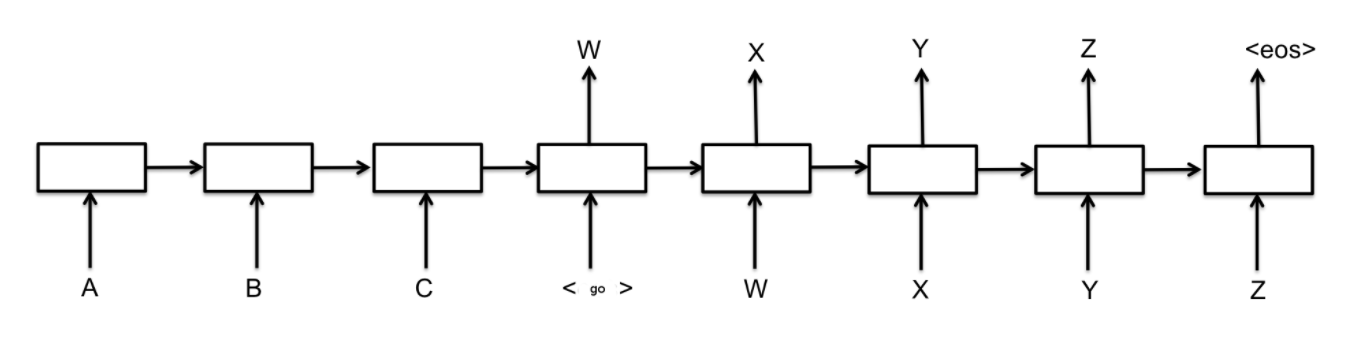
\includegraphics[scale=0.5]{seq2seq} \newline
\textit{Figure x: Sequence to Sequence, from Tensorflow \cite{seq2seq}. Each box in the picture above represents a cell of the RNN } \newline

We mentioned in the section about RNN that a network can learn to model a language**(TODO). In this section we describe the Sequence to Sequence model, which can generate a meaningful based on some given input. The sequence to sequence model is often referred to as an Encoder-Decoder architecture, as it consists of two RNNs: an encoder that processes the input and a decoder that generates the output. Encoder and decoder can share weights or use a different set of parameters

In the following sub sections we will describe the most common cells used for Sequence to Sequence modelling, and further look at extensions of these cell. 

\subsection{LSTM}
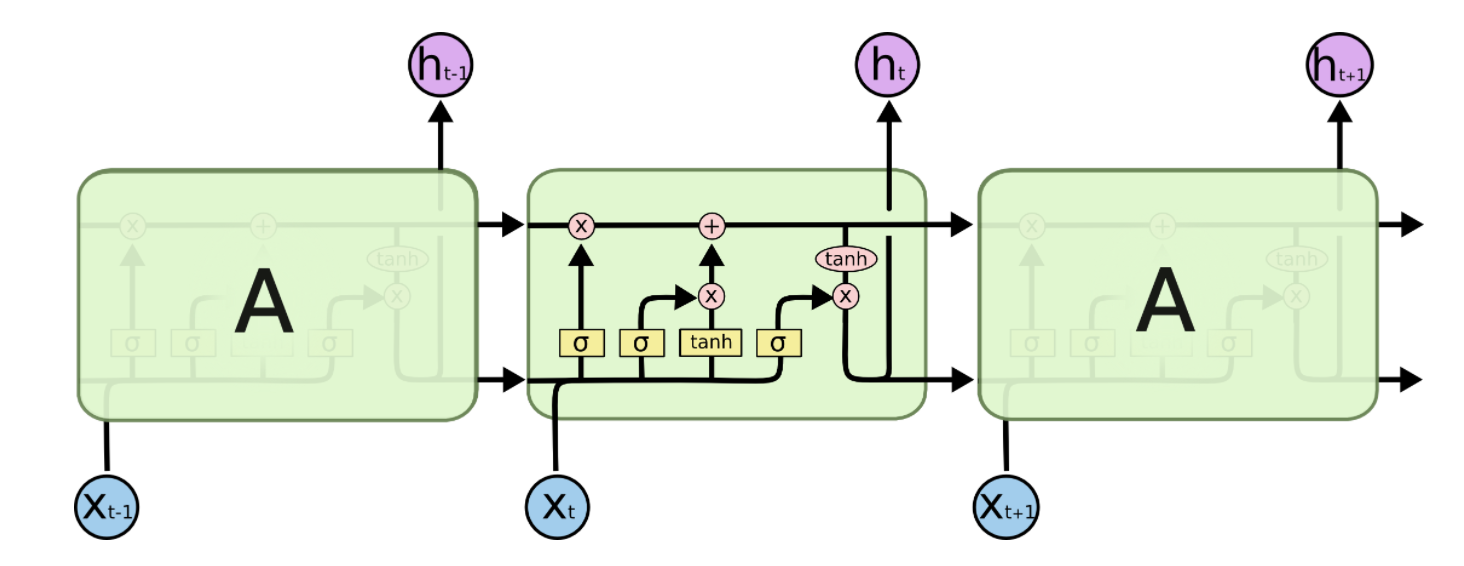
\includegraphics[scale=0.5]{lstm_cells} \newline
\textit{Figure 1: LSTM cells. TODO: change figure so that it is easy to see the forget gate etc.. } \newline

Long short-term memory (LSTM) is an RNN architecture first proposed in 1997 \cite{LSTM} which has been increasingly popular after its origin. The LSTMs are able to learn long term dependencies in a greater extent than before. The layer in each repeating module in the RNN is replaced with a LSTM cell and this is where the magic happens. The most important in the LSTM cell is the state. This is like a conveyor belt where the history on it may or may not be affected by new data fed into the module. The change of the state is dependent of the three gates the cell is built up of. First, we have the \textit{forget gate} which decides how much of the old history in the state that should be carried on. All of the gates consists of a sigmoid function outputs values between zero and one. If the forget gate outputs a value of one, it indicates that the all of the history should go through, while a value of zero means that nothing should pass. The second gate, the input gate, decides how much of the new stuff, the input, that should be added to the state. Values close to one means that all of the input should be added. Finally the output gate tells how much of the state that we should output.

\subsection{GRU}
The resent years, Gated Recurrent Units (GRU), have been very popular as an alternative to the LSTM. The cell consists of only two gates, \textit{reset} and \textit{update} gate. By reducing the number of gates, the model becomes easier to train and hence we get a performance gain, as well as it is easier to implement. Since it first use in 2004 \cite{Cho} it has shown good results, though it is performing slightly worse than LSTM, but the reduce in complexity has made it to a popular choice. However, the architecture is still new and not as good researched as LSTMs, which may result in discovering new drawbacks during the next years.

\subsection{Stacked LSTM}
As the popularity of the LSTMs increased, different setups of the cell and the network were tested out. Stacked LSTM is really similar to the standard LSTM, and the only difference is that there are several layers stacked on top of each other \cite{gridLSTM}. This means that the output from one layer of LSTM cells will go directly into another layer of LSTM cells.

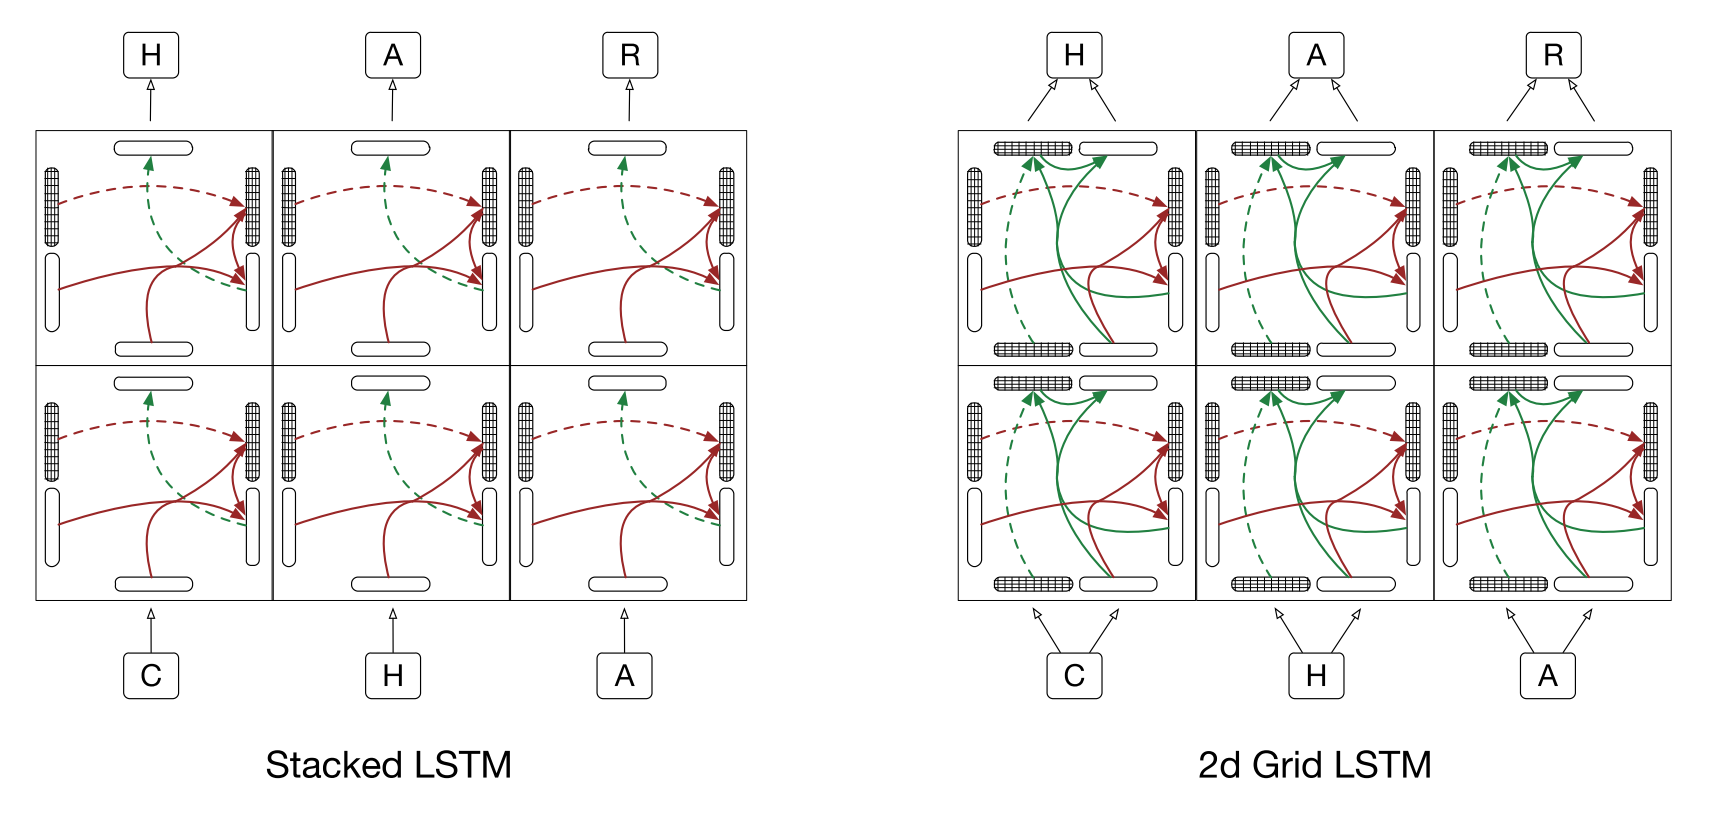
\includegraphics[scale=0.4]{stacked_vs_2dgrid} \newline
\textit{Figure 2**: Stacked LSTM vs 2D-Grid LSTM. Each block consists of several LSTM cells (Shaded rectangles). The 2D-Grid LSTM has LSTM cells along the depth dimension too, i.e. the layers are also connected. **Confuisng figure, make a new one}

\subsection{Grid LSTM}
The Grid LSTM is an extension of the LSTM cell, and a network (Kalchbrenner et al) \cite{Kalchbrenner} proposed in 2016**(version3)**. It is simply a network of LSTM cells arranged in a multidimensional grid. The network differs from existing deep LSTM architectures in that the depth dimension is treated like the other dimensions. Meaning that the cells are connected between the layers, and not just within the layers. TODO: What is the goal.**

One dimensional Grid LSTM is analogous to a feed-forward network that uses LSTM cells. Two dimensional Grid LSTM corresponds to the Stacked LSTM (A network with multiple LSTM layers), but it adds cells along the depth dimension too. If we have three or more dimensions, we have a Multidimensional LSTM, but it differs from this model by having the cells along the depth dimension, as well as we have a N-way interaction that is not prone to the instability present in Multi-Dimensional LSTM.**


\subsubsection{Blocks}
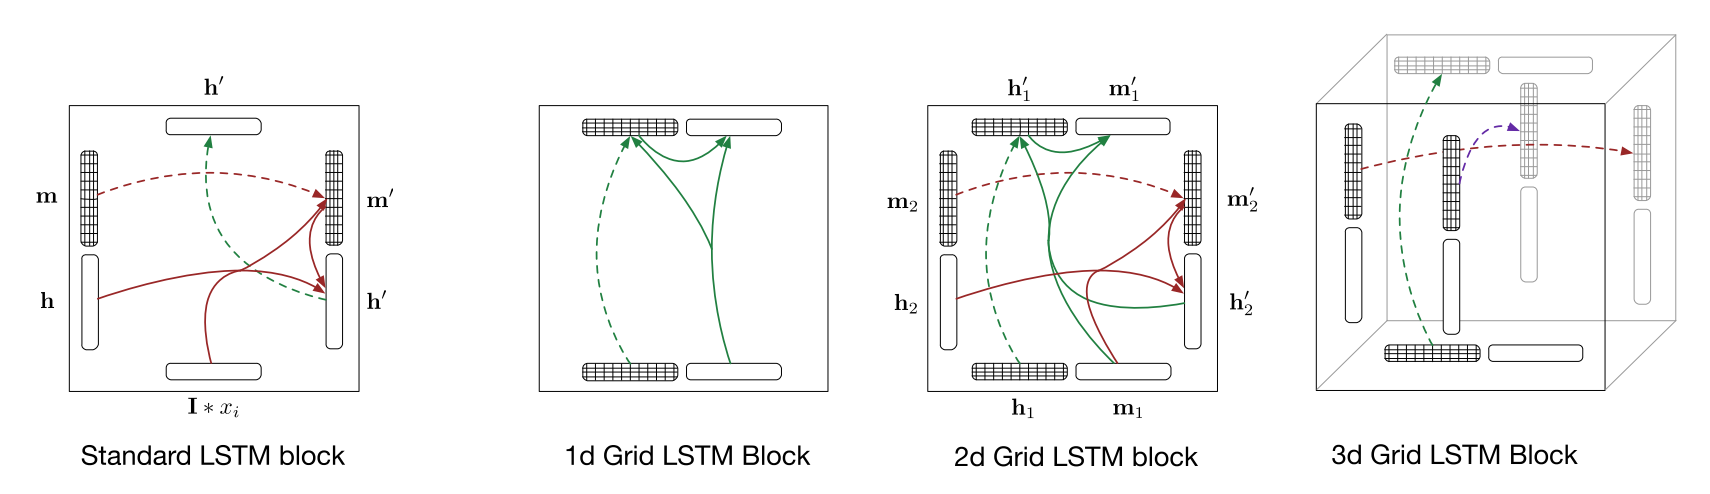
\includegraphics[scale=0.4]{gridblocks} \newline
\textit{Figure 3**: The structure of different blocks}

 When we talk about the Grid LSTM, we say that the architecture consists of several blocks. The structure of the blocks for different networks are illustrated in figure XX**. The standard LSTM block has one LSTM cell, i.e. it has a self loop and it can output the hidden state. The 1D Grid LSTM does not have any self loops, as it is only a cell in a feed-forward network and it is not recurrent. The 2D Grid LSTM block consists of two LSTM cells, one operates in the vertical dimension** (as in an ordinary LSTM) and the other cell (operates in the horizontal dimension) or (operates in the depth, connecting the different layers)**. The 3D Grid LSTM operates in one additional dimension.** 


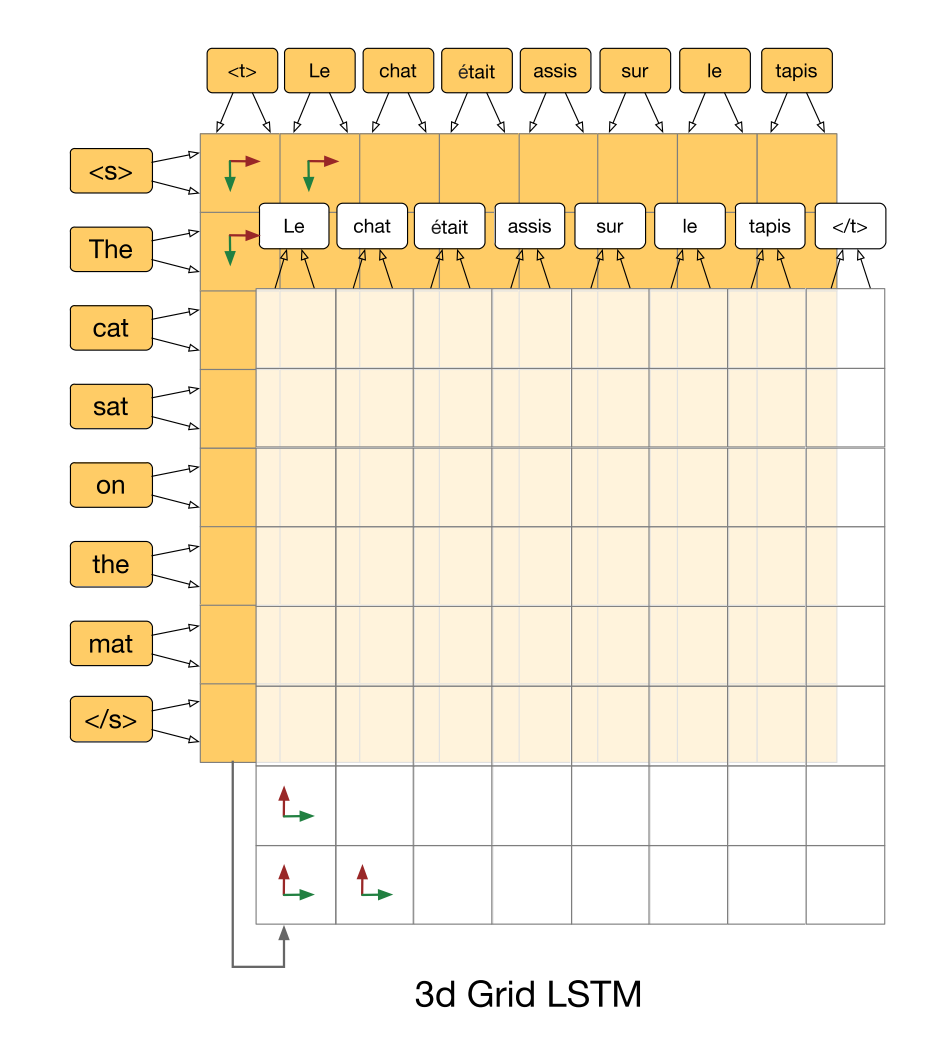
\includegraphics[scale=0.5]{3dgridlstm} \newline
\subsubsection{Grid LSTM Architecture for Sequence}
 Because we study a sequence, the 2D-Grid LSTM is of our interest. The model used for the translation problem in \cite{Kalchbrenner} uses one dimension to process the source sentence whereas the other dimension produces the target sentence. The network will repeatedly scan the source sentence for each generated target word. Two stacked two-dimensional grids, operating in the opposite directions, is used to increase capacity and help with learning longer scale translation patterns by giving us a bidirectional processing. The resulting model is a three-dimensional Grid LSTM where hierarchy grows along the third dimension (the depth of the network). The block in a Grid LSTM receives N hidden vectors $h_1, ..., h_N$ as well as N memory vectors $m'_1, ..., m'_N$ as input, just as for multidimensional LSTM where the the block consists of N dimensions. The block outputs, however, N hidden vectors and N memory vectors that are all very distinct. The block will then compute one transform LSTM for each dimension. **Write more

%-----

%Grid LSTM is a network of LSTM cells arranged in a grid of one or more dimensions \cite{gridLSTM}. This is analogues to the stacked LSTM, just with the possibility to add cells along the depth dimension too. A grid LSTM with three or more dimensions, on the other hand, equals a multidimensional LSTM, but with the possibility of having cells not just along the depth dimension.

%The grid LSTM have proven better results than ordinary LSTMs in the context of translation of languages \cite{gridLSTM}. Keeping this in mind, there is a reason to believe that grid LSTM will do good in the use of a chatbot.

%Skal mest sannsynlig fjernes
%\section{How to combine retrieval and generative models}
%The difference between the retrieval and generative models are obvious, as we state in section 4 in "The Current State of Art". The first will pick a response from a fixed set, and the latter will generate new and possible unseen responses. There are pros and cons with both models. The retrieval model is not flexible enough to be used for an expandable open domain conversational system. The generative model may have grammatically or linguistic errors, and the structure of the sentence may not make sense at all. There have not been proposed any papers on how we can extract the "best from both worlds". 

%In this phase of the project, we could implement both a generative and a retrieval based model, and compare the outputs with a scoring algorithm and show the best answer to the user. However, there are a lot of challenges due to this. First of all, for each incoming sequence, we will need to traverse two different neural networks and then run a comparable algorithm which will be time consuming. The training time will be doubled, and how should we create a scoring metrics to decide whether the retrieval one or the generative one is the best?

%An other interesting approach could be to somehow use the retrieval one to build the sentence structure, and then further fill in the words from the generative model. This could remove a lot of the grammatical errors, but would need the model to understand which part of speech each word belongs to. The challenges around this is probably beyond our knowledge.

%--------------------


\section{Challenges}
\begin{itemize}
    \item TBA
    \item TBA 
\end{itemize}

\section{Experimental part}
TBA
Test 
\section{Exploring data sets}

\begin{itemize}
    \item WMT'14 Translation Data set (Sequence to Sequence Paper). Open source.
   % \item Telenor customer chat. Private (KANSKJE TIL MASTER, MEN IKKE TIL PROSJEKTOPPGAVE)
    \item Ubuntu Dialogue Corpus. Open source
\end{itemize}

\section{The road ahead}
TBA

\section{Conclusion}
TBA
\section{Acknowledgment}
TBA
\begin{thebibliography}{1}
\bibitem{Graves}
[Graves et al. v1 2007] Multi-Dimensional Recurrent Neural Networks
\bibitem{Bahdanau}
[Bahdanau et al. v7 2016] http://arxiv.org/abs/1409.0473v3
\bibitem{Dodge}
[Dodge et al. v6 2016] http://arxiv.org/pdf/1511.06931v6.pdf
\bibitem{Lowe}
[Lowe et al. v3 2016] https://arxiv.org/pdf/1506.08909.pdf
\bibitem{Shang}
[Shang et al. v2 2015] https://arxiv.org/pdf/1503.02364.pdf
\bibitem{Vinyals}
[Vinyals et al. v3 2015] http://arxiv.org/pdf/1506.05869v3.pdf
\bibitem{Cho}
[Cho et al. v3 2014] https://arxiv.org/pdf/1406.1078v3.pdf
\bibitem{Sutskever}
[Sutskever et al. v3 2014] https://arxiv.org/pdf/1409.3215v3.pdf
\bibitem{Kalchbrenner}
[Kalchbrenner et al 2016] https://arxiv.org/pdf/1507.01526.pdf
\bibitem{Normalizer}
[Github] https://github.com/superscriptjs/normalizer
\bibitem{NLTK}
[Bird, Steven, Edward Loper and Ewan Klein (2009), Natural Language Processing with Python. O’Reilly Media Inc.] http://www.nltk.org/
\bibitem{LSTM}
[Hockreiter \& Schimhuber 1997] http://deeplearning.cs.cmu.edu/pdfs/Hochreiter97\_lstm.pdf
\bibitem{gridLSTM}
[Kalchbrenner et al. v3 2016] https://arxiv.org/pdf/1507.01526.pdf
\bibitem{seq2seq}
Sequence to Sequence model by Tensorflow. https://www.tensorflow.org/versions/r0.11/tutorials/seq2seq/index.html\#sequence-to-sequence-models

\end{thebibliography} http://arxiv.org/abs/0705.2011
\end{document}
